\documentclass[a4paper]{article}

\usepackage[utf8]{inputenc}
\usepackage[portuguese]{babel}
\usepackage{a4wide}
\usepackage[pdftex]{hyperref}
\usepackage{graphicx}
\usepackage{wrapfig}
\usepackage{amsmath}
\usepackage{verbatim}
\usepackage{caption}
\usepackage{subcaption}
\usepackage{float}



\begin{document}

\begin{titlepage}
\begin{center}



\includegraphics[width=0.6\textwidth]{logo.jpg}\\[0.5cm]

{\large Universidade do Minho - Escola de Engenharia}\\[0.5cm]

{\large Relatório do trabalho prático de Sistemas Distribuídos}\\[0.5cm]

% Title
\rule{\linewidth}{0.5mm} \\[0.4cm]
{ \huge \bfseries Matchmaking num jogo online \\[0.4cm] }
\rule{\linewidth}{0.5mm} \\[1.5cm]

% Author and supervisor
\noindent
\begin{minipage}{0.4\textwidth}
  \begin{flushleft} \large
    \emph{Autores :}\\
    Daniel Maia \textsc{(A77531)}\\
    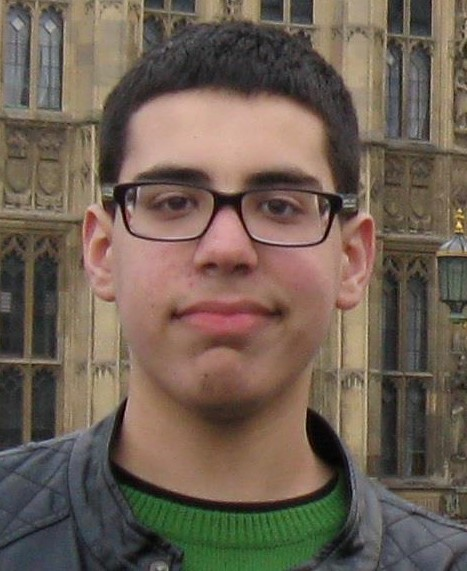
\includegraphics[width=1.5cm]{daniel.jpg}\break
    Diogo Silva\textsc{(A78034)}\\
    
\includegraphics[width=1.5cm]{afonso.jpg}\break
    Marco Silva\textsc{(A79607)}\\
    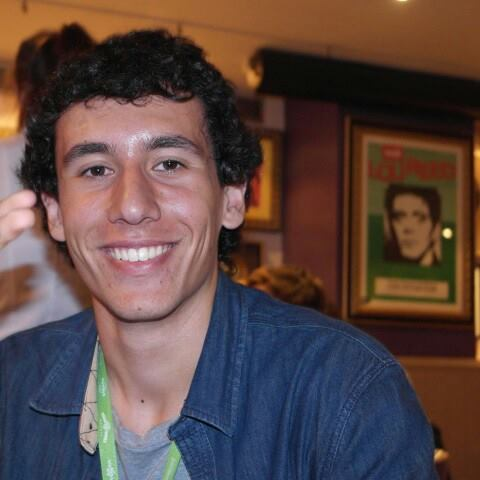
\includegraphics[width=1.5cm]{marco.jpg}\break
  \end{flushleft}
\end{minipage}%
\vfill

% Bottom of the page
{\large Versão 1.0 \\ \today}

\end{center}
\end{titlepage}




\begin{abstract}

\hspace{3mm} 

\end{abstract}

\pagebreak
\tableofcontents

\pagebreak
\section{Introdução}
\label{sec:1}

\hspace{3mm} 



%------------------------------------------------------------------------

\pagebreak
\section{Descrição do problema}
\label{sec:2}

\hspace{3mm} A proposta de trabalho dada para o projeto é o da implementação de uma aplicação distribuída para \textit{matchmaking} num jogo \textit{online}, num estilo semelhante a videojogos tais como Overwatch ou Paladins. Esta aplicação terá a capacidade de, nomeadamente, formar automaticamente duas equipas por partida e permitir a cada jogador um intervalo de tempo para escolher uma personagem, referida como herói, antes da partida iniciar.

\par Cada equipa será constituída por 5 jogadores, cada um com uma classificação pessoal. Esta classificação, determinada pelas vitórias e derrotas sofridas no jogo, terá um valor inteiro entre 0 e 9, e terá no máximo uma diferença unitária entre todos os jogadores de uma dada partida. Tendo encontrado 10 jogadores disponíveis com classificações semelhantes, o servidor dividi-los-á em equipas equilibradas de acordo com as classificações dos mesmos. Para que esta classificação seja guardada, será implementado um sistema de registo e autenticação. Com um nome de utilizador e uma palavra passe, o servidor autentica o jogador sempre que este estabelece ligação ao mesmo.

\par Tendo as duas equipas feitas, os jogadores procederão à fase da escolha dos heróis, dos quais existem 30. Cada jogador poderá escolher qualquer um, desde que este não tenha ainda sido selecionado por outro jogador da mesma equipa. Como tal, cada jogador poderá ver as escolhas de heróis dos elementos da mesma equipa. Qualquer jogador poderá selecionar um herói diferente, caso mude de ideias. Após 30 segundos, a fase de escolha será dada como terminada. Se algum jogador da partida não tiver escolhido um herói, a partida é abortada e cada jogador terá de selecionar a opção de jogar uma vez mais. Caso contrário, será mostrada a composição de ambas equipas a todos os jogadores da partida, nomeadamente o nome de utilizador de cada jogador e respetivo herói. É depois simulada uma partida, cujo resultado aleatório será utilizado para atualizar a classificação de cada jogador, subindo com cada vitória e descendo com cada derrota.

\par Para aceder ao servidor, cada jogador terá acesso a um programa Cliente, com o qual acederá a um Servidor \textit{multithreaded} através de \textit{sockets} TCP. Em concordância com a proposta do trabalho, o protocolo entre os dois será baseado em texto, orientado à linha, e cada \textit{thread} do Servidor escreverá em um e só um \textit{socket}.


\pagebreak
\clearpage
%--------------------------------------------------------------------------

\section{Conceção da Solução}
\label{sec:3}

\subsection{Registo e login}

\hspace{3mm} 



\subsection{Matchmaking}

\hspace{3mm} 




\subsection{Fazer equipas}

\hspace{3mm} 

\subsection{Escolha de heróis}

\hspace{3mm} 

\subsection{Cálculo dos resultados}

\hspace{3mm} 

\pagebreak

%--------------------------------------------------------------------------

\section{Conclusões}
\label{sec:4}

\hspace{3mm} 



\end{document}
